\documentclass{standalone}
\usepackage{tikz}
\usetikzlibrary{patterns, positioning}

\begin{document}
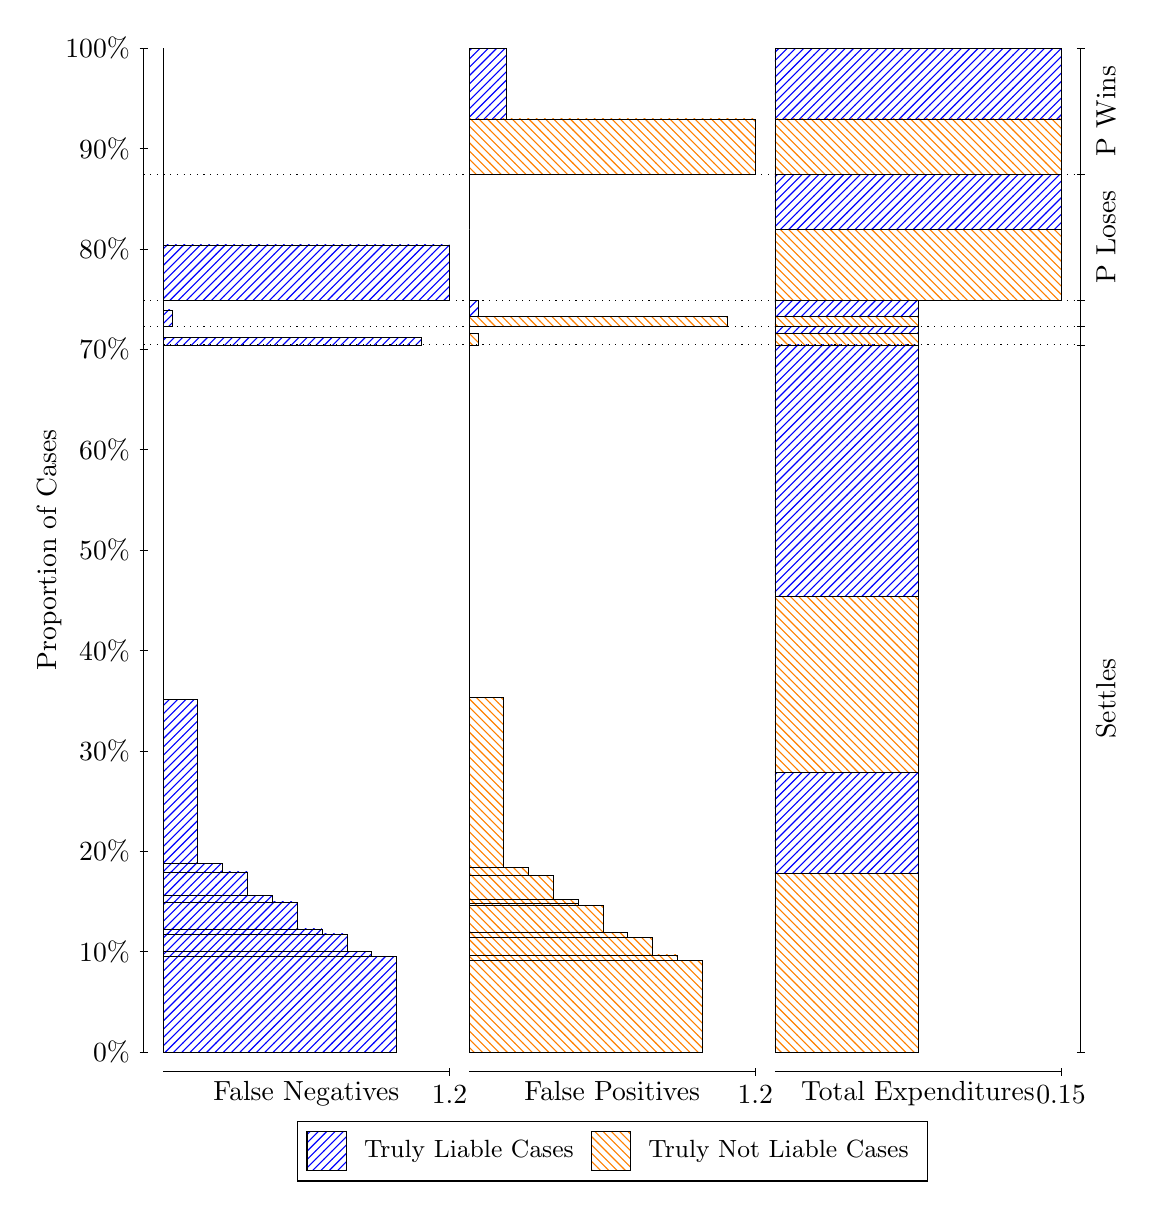
\begin{tikzpicture}
\draw[black, very thin] (1.5,1.75) -- (1.5,14.5);
\node[rotate=90, anchor=center] at (0.3, 8.125) {Proportion of Cases};
\draw[black, very thin] (1.45,1.75) -- (1.55,1.75);
\node[anchor=east] at (1.45, 1.75) {0\%};
\draw[black, very thin] (1.45,3.025) -- (1.55,3.025);
\node[anchor=east] at (1.45, 3.025) {10\%};
\draw[black, very thin] (1.45,4.3) -- (1.55,4.3);
\node[anchor=east] at (1.45, 4.3) {20\%};
\draw[black, very thin] (1.45,5.575) -- (1.55,5.575);
\node[anchor=east] at (1.45, 5.575) {30\%};
\draw[black, very thin] (1.45,6.85) -- (1.55,6.85);
\node[anchor=east] at (1.45, 6.85) {40\%};
\draw[black, very thin] (1.45,8.125) -- (1.55,8.125);
\node[anchor=east] at (1.45, 8.125) {50\%};
\draw[black, very thin] (1.45,9.4) -- (1.55,9.4);
\node[anchor=east] at (1.45, 9.4) {60\%};
\draw[black, very thin] (1.45,10.675) -- (1.55,10.675);
\node[anchor=east] at (1.45, 10.675) {70\%};
\draw[black, very thin] (1.45,11.95) -- (1.55,11.95);
\node[anchor=east] at (1.45, 11.95) {80\%};
\draw[black, very thin] (1.45,13.225) -- (1.55,13.225);
\node[anchor=east] at (1.45, 13.225) {90\%};
\draw[black, very thin] (1.45,14.5) -- (1.55,14.5);
\node[anchor=east] at (1.45, 14.5) {100\%};

\draw[black, very thin] (13.4,1.75) -- (13.4,14.5);
\draw[black, very thin] (13.35,1.75) -- (13.45,1.75);
\node[anchor=west] at (13.35, 1.75) {};
\draw[black, very thin] (13.35,10.73) -- (13.45,10.73);
\node[anchor=west] at (13.35, 10.73) {};
\draw[black, very thin] (13.35,10.969) -- (13.45,10.969);
\node[anchor=west] at (13.35, 10.969) {};
\draw[black, very thin] (13.35,11.299) -- (13.45,11.299);
\node[anchor=west] at (13.35, 11.299) {};
\draw[black, very thin] (13.35,12.898) -- (13.45,12.898);
\node[anchor=west] at (13.35, 12.898) {};
\draw[black, very thin] (13.35,14.5) -- (13.45,14.5);
\node[anchor=west] at (13.35, 14.5) {};

\draw[black, very thin, pattern color=blue, pattern=north east lines] (1.75,1.75) rectangle (4.712,2.9598);
\draw[black, very thin, pattern color=blue, pattern=north east lines] (1.75,2.9598) rectangle (4.396,3.0298);
\draw[black, very thin, pattern color=blue, pattern=north east lines] (1.75,3.0298) rectangle (4.0801,3.2503);
\draw[black, very thin, pattern color=blue, pattern=north east lines] (1.75,3.2503) rectangle (3.7641,3.3128);
\draw[black, very thin, pattern color=blue, pattern=north east lines] (1.75,3.3128) rectangle (3.4482,3.657);
\draw[black, very thin, pattern color=blue, pattern=north east lines] (1.75,3.657) rectangle (3.1322,3.734);
\draw[black, very thin, pattern color=blue, pattern=north east lines] (1.75,3.734) rectangle (2.8163,4.0385);
\draw[black, very thin, pattern color=blue, pattern=north east lines] (1.75,4.0385) rectangle (2.5004,4.1423);
\draw[black, very thin, pattern color=blue, pattern=north east lines] (1.75,4.1423) rectangle (2.1844,6.2252);
\draw[black, very thin, pattern color=orange, pattern=north west lines] (1.75,6.2252) rectangle (1.75,10.73);
\draw[black, very thin, pattern color=blue, pattern=north east lines] (1.75,10.73) rectangle (5.0279,10.823);
\draw[black, very thin, pattern color=orange, pattern=north west lines] (1.75,10.823) rectangle (1.75,10.969);
\draw[black, very thin, pattern color=blue, pattern=north east lines] (1.75,10.969) rectangle (1.8685,11.175);
\draw[black, very thin, pattern color=orange, pattern=north west lines] (1.75,11.175) rectangle (1.75,11.299);
\draw[black, very thin, pattern color=blue, pattern=north east lines] (1.75,11.299) rectangle (5.3833,12.001);
\draw[black, very thin, pattern color=orange, pattern=north west lines] (1.75,12.001) rectangle (1.75,12.898);
\draw[black, very thin, pattern color=orange, pattern=north west lines] (1.75,12.898) rectangle (1.75,13.601);
\draw[black, very thin, pattern color=blue, pattern=north east lines] (1.75,13.601) rectangle (1.75,14.5);
\draw[black, very thin, pattern color=orange, pattern=north west lines] (5.6333,1.75) rectangle (8.5953,2.9147);
\draw[black, very thin, pattern color=orange, pattern=north west lines] (5.6333,2.9147) rectangle (8.2793,2.9834);
\draw[black, very thin, pattern color=orange, pattern=north west lines] (5.6333,2.9834) rectangle (7.9634,3.2081);
\draw[black, very thin, pattern color=orange, pattern=north west lines] (5.6333,3.2081) rectangle (7.6475,3.2716);
\draw[black, very thin, pattern color=orange, pattern=north west lines] (5.6333,3.2716) rectangle (7.3315,3.6153);
\draw[black, very thin, pattern color=orange, pattern=north west lines] (5.6333,3.6153) rectangle (7.0156,3.642);
\draw[black, very thin, pattern color=orange, pattern=north west lines] (5.6333,3.642) rectangle (7.0156,3.6903);
\draw[black, very thin, pattern color=orange, pattern=north west lines] (5.6333,3.6903) rectangle (6.6996,3.9885);
\draw[black, very thin, pattern color=orange, pattern=north west lines] (5.6333,3.9885) rectangle (6.3837,4.0935);
\draw[black, very thin, pattern color=orange, pattern=north west lines] (5.6333,4.0935) rectangle (6.0678,6.2548);
\draw[black, very thin, pattern color=blue, pattern=north east lines] (5.6333,6.2548) rectangle (5.6333,10.73);
\draw[black, very thin, pattern color=orange, pattern=north west lines] (5.6333,10.73) rectangle (5.7518,10.876);
\draw[black, very thin, pattern color=blue, pattern=north east lines] (5.6333,10.876) rectangle (5.6333,10.969);
\draw[black, very thin, pattern color=orange, pattern=north west lines] (5.6333,10.969) rectangle (8.9112,11.093);
\draw[black, very thin, pattern color=blue, pattern=north east lines] (5.6333,11.093) rectangle (5.7518,11.299);
\draw[black, very thin, pattern color=orange, pattern=north west lines] (5.6333,11.299) rectangle (5.6333,12.197);
\draw[black, very thin, pattern color=blue, pattern=north east lines] (5.6333,12.197) rectangle (5.6333,12.898);
\draw[black, very thin, pattern color=orange, pattern=north west lines] (5.6333,12.898) rectangle (9.2667,13.601);
\draw[black, very thin, pattern color=blue, pattern=north east lines] (5.6333,13.601) rectangle (6.1072,14.5);
\draw[black, very thin, pattern color=orange, pattern=north west lines] (9.5167,1.75) rectangle (11.333,4.0162);
\draw[black, very thin, pattern color=blue, pattern=north east lines] (9.5167,4.0162) rectangle (11.333,5.296);
\draw[black, very thin, pattern color=orange, pattern=north west lines] (9.5167,5.296) rectangle (11.333,7.5346);
\draw[black, very thin, pattern color=blue, pattern=north east lines] (9.5167,7.5346) rectangle (11.333,10.73);
\draw[black, very thin, pattern color=orange, pattern=north west lines] (9.5167,10.73) rectangle (11.333,10.876);
\draw[black, very thin, pattern color=blue, pattern=north east lines] (9.5167,10.876) rectangle (11.333,10.969);
\draw[black, very thin, pattern color=orange, pattern=north west lines] (9.5167,10.969) rectangle (11.333,11.093);
\draw[black, very thin, pattern color=blue, pattern=north east lines] (9.5167,11.093) rectangle (11.333,11.299);
\draw[black, very thin, pattern color=orange, pattern=north west lines] (9.5167,11.299) rectangle (13.15,12.197);
\draw[black, very thin, pattern color=blue, pattern=north east lines] (9.5167,12.197) rectangle (13.15,12.898);
\draw[black, very thin, pattern color=orange, pattern=north west lines] (9.5167,12.898) rectangle (13.15,13.601);
\draw[black, very thin, pattern color=blue, pattern=north east lines] (9.5167,13.601) rectangle (13.15,14.5);
\draw[black, dotted] (1.5,10.73) -- (13.4,10.73);
\draw[black, dotted] (1.5,10.969) -- (13.4,10.969);
\draw[black, dotted] (1.5,11.299) -- (13.4,11.299);
\draw[black, dotted] (1.5,12.898) -- (13.4,12.898);
\draw[black, very thin] (1.75,1.5) -- (5.3833,1.5);
\node[anchor=north] at (3.5667, 1.5) {False Negatives};
\draw[black, very thin] (5.3833,1.45) -- (5.3833,1.55);
\node[anchor=north] at (5.3833, 1.45) {1.2};

\draw[black, very thin] (5.6333,1.5) -- (9.2667,1.5);
\node[anchor=north] at (7.45, 1.5) {False Positives};
\draw[black, very thin] (9.2667,1.45) -- (9.2667,1.55);
\node[anchor=north] at (9.2667, 1.45) {1.2};

\draw[black, very thin] (9.5167,1.5) -- (13.15,1.5);
\node[anchor=north] at (11.333, 1.5) {Total Expenditures};
\draw[black, very thin] (13.15,1.45) -- (13.15,1.55);
\node[anchor=north] at (13.15, 1.45) {0.15};

\node[black, centered, rotate=90] at (13.72, 6.24) {Settles};


\node[black, centered, rotate=90] at (13.72, 12.099) {P Loses};
\node[black, centered, rotate=90] at (13.72, 13.699) {P Wins};

\draw (7.449999999999999,1.5) node[draw=none] (baseCoordinate) {};
\begin{scope}[align=center]
        \matrix[scale=0.5, draw=black, below=0.5cm of baseCoordinate, nodes={draw}, column sep=0.1cm]{
            \node[rectangle, draw, minimum width=0.5cm, minimum height=0.5cm, pattern=north east lines, pattern color=blue] {}; &
            \node[draw=none, font=\small] (B) {Truly Liable Cases}; &
            \node[rectangle, draw, minimum width=0.5cm, minimum height=0.5cm, pattern=north west lines, pattern color=orange] {}; &
            \node[draw=none, font=\small] (B) {Truly Not Liable Cases}; \\
            };
\end{scope}

\end{tikzpicture}
\end{document}